% 2006 年上海春季卷第 21 题（1）：独立解答函数图。
% 与题面空白网格分开；按 f(x)=|x^2-4x-5| 在 [-2,6] 上作图。
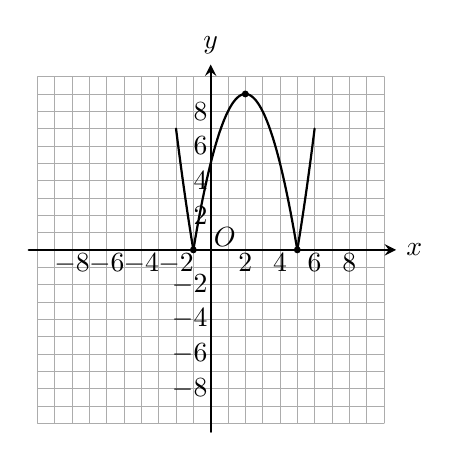
\begin{tikzpicture}[line cap=round,line join=round,x=0.22cm,y=0.22cm,>=stealth]
  \draw[step=1,gray!65,very thin] (-10,-10) grid (10,10);
  \draw[->,thick] (-10.5,0)--(10.7,0) node[right] {$x$};
  \draw[->,thick] (0,-10.5)--(0,10.7) node[above] {$y$};

  \foreach \x in {-8,-6,-4,-2,2,4,6,8}
    \node[below,inner sep=1pt] at (\x,0) {$\x$};
  \foreach \y in {-8,-6,-4,-2,2,4,6,8}
    \node[left,inner sep=1pt] at (0,\y) {$\y$};
  \node[above right,inner sep=1pt] at (0,0) {$O$};

  \draw[thick,domain=-2:-1,samples=40,variable=\x]
    plot (\x,{\x*\x-4*\x-5});
  \draw[thick,domain=-1:5,samples=100,variable=\x]
    plot (\x,{-\x*\x+4*\x+5});
  \draw[thick,domain=5:6,samples=40,variable=\x]
    plot (\x,{\x*\x-4*\x-5});
  \fill (-1,0) circle (1.25pt);
  \fill (2,9) circle (1.25pt);
  \fill (5,0) circle (1.25pt);
\end{tikzpicture}
